\section{Versuchsziel}
{\footnotesize \textit{Carl Arne Thomann}}

Es wird die effektive Masse von Elektronen in einem Material durch Ausnutzen des Faraday-Effektes bestimmt.
\section{Theorie}
\label{sec:Theorie}
\subsection{Effektive Masse}
Die effektive Masse ist ein Konzept aus der Festkörperphysik,
um die im Allgemeinen komplizierte Dispersionsrelation - und damit das Verhalten - von Elektronen im Halbleitern
durch das Modell der freien Elektronen zu beschreiben.
Eine beispielhafte Dispersionsrelation von Elektronen im Halbleitern ist in
Abbildung \ref{fig:dispersion} gezeigt.
\begin{figure}
    \centering
    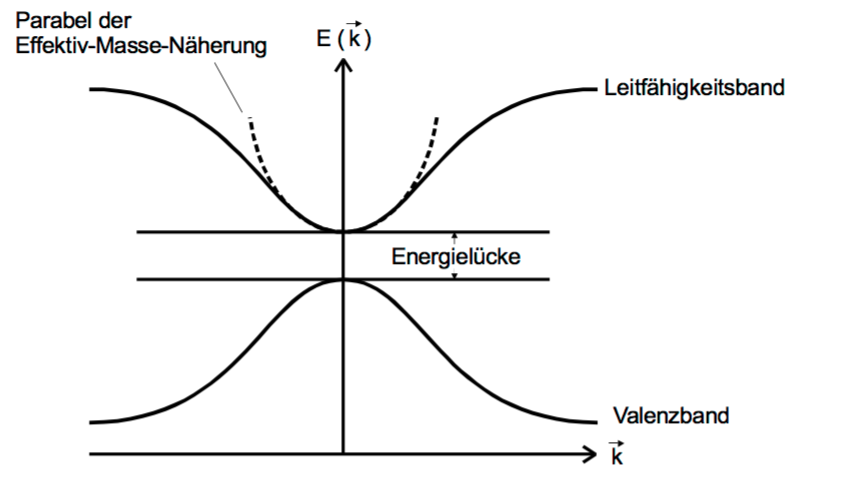
\includegraphics[width=0.8\textwidth]{graphics/dispersion.png}
    \caption{Beispiel einer Dispersionsrelation für Elektronen eines Halbleiters mit Parabel-Näherung. Charakteristisch ist die Bandlücke (hier: Energielücke) zwischen Valnezband und Leitungsband (hier: Leitfähigkeitsband). \cite{skript}}
    \label{fig:dispersion}
\end{figure}
Wird am $\Gamma$\-/Punkt ($|\vec k| = 0$) die Dispersion durch eine Parabel angenährt,
\begin{equation}
    E(\vec k) = E(0) + \frac{1}{2}\sum\limits_{i=1}^3 \frac{\partial^2 E}{\partial k_i^2}\Bigl|_{x=0}k_i^2,
\end{equation}
und mit der Energiedispersion freier Elektronen verglichen, %die anstelle der Ruhemasse $m_0$ eine modifizierte Masse $m^{*}$ tragen,
\begin{equation}
    E(\vec k) = \frac{h^2}{(2\pi)^2}\frac{k^2}{2m},
\end{equation}
kann ein Halbleiterelektronen als freies Elektron beschrieben werden, sofern die Masse des freien Halbleiterelektrons als
\begin{equation}
    m = \frac{h}{(2\pi)^2}\frac{1}{\frac{\partial^2 E}{\partial k_i^2}\Bigl|_{k=0}}
\end{equation}
festgesetzt wird.
Mit dieser effektiven Masse gehen vorherige Gleichungen ineinander über und die Konzepte vereinen.
Für symmetrische Halbleiter ist die Unterscheidung der drei Richtungen $k_i$ überflüssig;
es wird von kugelförmigen Energieflächen gesprochen.
\begin{equation}
    E(\vec k) = E(0) + \frac{h^2}{(2\pi)^2}\frac{k^2}{2m}
\end{equation}
\subsection{Zirkulare Doppelbrechung von optisch aktiven Medien}
\label{sec:doppel_aktiv}
Zirkulare Doppelbrechung beschreibt die Abhängigkeit des Brechungsindex von der Polarisation mit dem Effekt,
linear polarisiertes Licht bei der Transmission durch den Kristall um den sogenannten Faraday-Winkel $\Theta$ zu drehen.
Die Ursache dafür liegt in elektrischen Dipolen, die einerseits in den Gitteratome und
andererseits durch Bandelektronen bei Wechselwirkung mit den Atomrümpfen induziert werden.
Linear polarisiertes Licht wird als Überlagerung von links- und rechtsdrehender zirkular polarisiertem Licht,
\begin{align}
    E(z) &= \frac{1}{2} \left(E_\text{R}(z)+E_\text{L}(z)\right)\\
    \shortintertext{mit}
    E_\text{R}(z) &= (E_0 \vec x_0 - i E_0 \vec y_0) \exp(ik_\text{R}z)\\
    E_\text{L}(z) &= (E_0 \vec x_0 + i E_0 \vec y_0) \exp(ik_\text{L}z).
\end{align}
\begin{figure}[h]
    \centering
    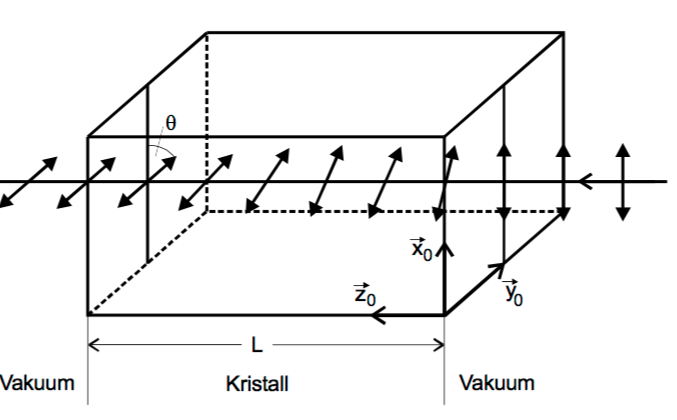
\includegraphics[width=0.8\textwidth]{graphics/drehung.png}
    \caption{Drehung der Polarisationsebene von linear püolarisiertem Licht bei Transmission durch ein optisch aktives Material. \cite{skript}}
    \label{fig:drehung}
\end{figure}
Die Polarisation des Lichtes beim Eintritt in das Medium wird als
\begin{equation}
    E(z=0) = E_0 \vec x_0
\end{equation}
festgelegt.
Für $z = L$, dem Ort des Austritts aus dem Kristall, gilt
\begin{alignat*}{3}
    E(z=L) &= \frac{E_0}{2} \{ (\exp(ik_\text{R}L)+\exp(ik_\text{L}L))\vec x_0 + (i\exp(ik_\text{L}L)-i\exp(ik_\text{R}L))\vec y_0\}\\
    &= \frac{E_0}{2} \vec x_0 \{ \exp(i(k_\text{R}+k_\text{L})\sfrac{L}{2})\exp(i(k_\text{R}-k_\text{L})\sfrac{L}{2}) \\
    &\phantom{=} + \exp(i(k_\text{R}+k_\text{L})\sfrac{L}{2})\exp(i(-k_\text{R}+k_\text{L})\sfrac{L}{2})\}\\
    &\phantom{=}+ \frac{E_0}{2}\vec y_0 \{ \exp(i(-k_\text{R}+k_\text{L})\sfrac{L}{2})\exp(i(k_\text{R}+k_\text{L})\sfrac{L}{2}) \\
    &\phantom{=}- \exp(i(k_\text{R}-k_\text{L})\sfrac{L}{2})\exp(i(k_\text{R}+k_\text{L})\sfrac{L}{2}) \}.
\end{alignat*}
Mit den Abkürzungen
\begin{align}
    \Psi &= \frac{L}{2} (k_\text{R}+k_\text{L})\\
    \Theta &= \frac{L}{2} (k_\text{R}-k_\text{L}) = \frac{L\omega}{2 c} (n_\text{R}-n_\text{L}) \label{eq:abk_theta}
\end{align}
ergibt sich schließlich für den austretenden Strahl
\begin{equation}
    E(z=L) = E_0 \exp(i\Psi)\begin{pmatrix} \cos(\Theta)\\\sin(\Theta)\end{pmatrix},
\end{equation}
eine um $\Theta$ gedrehte und um $\Psi$ phasenverschobene polarisierte Welle.
Bei angelegtem elektrischen Feld sei die Polarisation durch
\begin{equation}
    \vec P = \epsilon_0 \chi \vec E = \epsilon_0 \begin{pmatrix} \chi_{xx} & i\chi_{xy} & 0 \\ -i\chi_{xy} & \chi_{yy} & 0 \\ 0 & 0 & \chi_{zz} \end{pmatrix} \begin{pmatrix} E_x\\E_y\\E_z \end{pmatrix}
    \label{eq:polarisation}
\end{equation}
beschrieben.
Ein Material wird doppelbrechend, wenn der Dielektrizitätstensor $\chi$ nicht-diagonale Elemente hat, die zueinander komplex konjugiert sind.
Ist dies der Fall, existieren zwei Lösungen $k_{\pm}$ für die Wellengleichung des Lichtes in Materie,
\begin{align}
    \nabla\times(\nabla\times\vec E) &= -\frac{1}{c^2}(1+\chi)\frac{\partial^2 E}{\partial t^2}\label{eq:wellengleichung}\\
    \intertext{mit Ansatz linearer Welle:}
    \vec E &= \vec E_0 \exp(i(\vec k \cdot \vec r - \omega t))\\
    \shortintertext{und}
    \vec k &= k \vec z.
\end{align}
Die Lösung dieser Gleichung \eqref{eq:wellengleichung},
\begin{equation}
    k_\pm = \frac{\omega}{c}\sqrt{(1+\chi_{xx})\pm\chi_{xy}},
\end{equation}
ergibt sich aus der Koeffizientenmatrix für die $x$\-/, $y$\-/ und $z$\-/Komponenten.
Die beiden Geschwindigkeiten
\begin{align}
    v_\text{Ph,R}=\frac{c}{\sqrt{1+\chi_{xx}+\chi_{xy}}} \qquad v_\text{Ph,L}=\frac{c}{\sqrt{1+\chi_{xx}-\chi_{xy}}}
\end{align}
sind für $\chi_{xy}\neq0$ unterschiedlich groß und können dem links- und dem rechtsdrehenden Anteil zugeordnet werden.
Hierzu werden beide Lösungen $k_\pm$ jeweils in die $x$- und $y$-Komponenten der Gleichung \eqref{eq:wellengleichung}
eingesetzt.

Nach \eqref{eq:abk_theta} besteht unter Annahme $\chi_{xy} << 1 + \chi_{xx}$ der Zusammenhang
\begin{equation}
    \Theta \approx \frac{L\omega v_\text{Ph}}{2c^2}\chi_{xy} = \frac{L\omega}{2cn}\chi_{xy},
    \label{eq:theta}
\end{equation}
wobei $v_\text{ph} = \frac{c}{\sqrt{1+\chi_{xx}}}$ ausgenutzt wurde.
\subsection{Zirkulare Doppelbrechung durch Anlegen von äußeren Feldern}
Auch bei optisch inaktiven Materialen kann eine Drehung von linear polarisiertem Licht wie in Abschnitt \ref{sec:doppel_aktiv} beobachtet werden.
Die Kraftgleichung von Elektronen, auf die $\vec E$\-/ und $\vec B$\-/Felder sowie ein harmonisches Potential wirken,
\begin{equation}
    -m\omega^2\vec r + K \vec r = -e_0 \vec E + i e_0 \omega \vec r \times \vec B
    \label{eq:kraft}
\end{equation}
lässt sich mit dem Ansatz von reiner Verschiebungspolarisation
\begin{equation}
    \vec P = - N e_0 \vec r
    \label{eq:verschiebung}
\end{equation}
in eine vergleichbare Form zu \eqref{eq:polarisation} bringen.
Hierzu wird der Ausdruck der Verschiebungspolarisation \eqref{eq:verschiebung} in die Kraftgleichung \eqref{eq:kraft} gesetzt und das so erhaltene Gleichungssystem betrachtet.
Wird weiter der Suszeptibilitätstensor $\chi$ in der Gestalt
\begin{equation}
    \chi = \begin{pmatrix} \chi_{xx} & i\chi_{xy} & 0 \\ i\chi_{yx} & \chi_{yy} & 0\\ 0 & 0 & \chi_{zz} \end{pmatrix}
\end{equation}
sowie ein homogenes Magnetfeld in $z$-Richtung angenommen, kann durch Koeffizientenvergleich der $\vec E$-Feldkomponenten zum Einen die Forderung $i\chi_{xy}=-i\chi_{yx}$ und damit zum Anderen die feldinduzierte Doppelbrechung gezeigt werden.
Durch Auflösen nach $\chi_{xy}$ wird abschließend mithilfe von Gleichung \eqref{eq:theta}
\begin{equation}
    \Theta = \frac{e_0^3}{2\epsilon_0 c}\frac{1}{m^2} \frac{\omega^2}{(-\omega^2+\frac{k}{m})^2-(\frac{e_0}{m}\omega B)^2} \frac{NBL}{n}
    \label{theta_1}
\end{equation}
mit der Ladungsträgeranzahl $N$, dem Magnetfeld $B$, der Länge des Kristalls $L$, der Brechzahl $n$ gefunden.
Für die Frequenz $\omega$ wird die Kreisfrequenz des Lichtes angesetzt.
Mit den Bezeichungen Resonanzfrequenz $\omega_0^2 =\frac{k}{m}$ und Zyklotronfrequenz $\omega_C^2 =\frac{e_0^2}{m^2} B^2$ wird Ausdruck \eqref{theta_1} zu
\begin{equation}
    \Theta = \frac{e_0^3}{2\epsilon_0 c}\frac{1}{m^2} \frac{\omega^2}{(-\omega^2+\omega_0^2)^2-(\omega_c\omega)^2} \frac{NBL}{n}.
    \label{theta_2}
\end{equation}
Bei einer Messfrequenz $\omega << \omega_0$ und $(\omega_0^2-\omega^2)^2>>(\omega_c\omega)^2$ wird \eqref{theta_2} zu
\begin{equation}
    \Theta = \frac{2\pi^2 e_0^3 c}{\epsilon_0} \frac{1}{m^2} \frac{1}{\lambda^2\omega_0^4} \frac{NBL}{n}
\end{equation}
genährt.
Für freie Elektronen, wie für diese Zwecke angesetzt, werden harmonische Kräfte $K$ ignoriert und es wird
\begin{equation}
    \Theta = \frac{e_0^3}{8\pi^2\epsilon_0 c^3} \frac{1}{m^2} \lambda^2 \frac{NBL}{n}
	\label{eqn:formel}
\end{equation}
gefunden.
